%%=============================================================================
%% POC
%%=============================================================================

\chapter{Proof of concept}%
\label{ch:poc}

\section{Noodzaak voor een App: Voordelen van een mobiele applicatie als een ElderSpeak-monitor}

In de context van gezondheidszorg en sociale diensten, vooral bij het opleiden en uitrusten van studenten of zorgverleners in het omgaan met en communiceren met oudere individuen, speelt de integratie van technologie een cruciale rol. De ontwikkeling van een mobiele applicatie voor het monitoren en beheren van ElderSpeak is om meerdere redenen zeer voordelig:


\begin{enumerate}[label=\arabic*.]
    
    \item \textbf{Draagbaarheid:}\\
    Het meest opvallende voordeel van het gebruik van een mobiele applicatie is de draagbaarheid. Studenten en zorgverleners bewegen vaak door verschillende omgevingen - of het nu in onderwijsinstellingen, woonhuizen of tijdens dagelijkse zorgtaken is. Een mobiele applicatie stelt hen in staat om een krachtig controlegereedschap in hun zak te dragen. Deze mobiliteit maakt onmiddellijke toegang tot de functionaliteiten van de app mogelijk, zoals het opnemen van interacties en het in real-time analyseren van spraak, ongeacht hun locatie.
    
    \item \textbf{Onmiddellijke Resultaten:}\\
    Het gebruik van een mobiele applicatie voor ElderSpeak-monitoring maakt real-time analyse en feedback mogelijk. Zodra een interactie is opgenomen, kan de applicatie onmiddellijke feedback geven aan de gebruiker over de kwaliteit van hun communicatie. Deze onmiddellijke reactie is cruciaal voor leren en correctie ter plekke, waardoor studenten en zorgverleners snel hun communicatiestrategieën met ouderen kunnen aanpassen en verbeteren.
    
    
    \item \textbf{Verbeterde Gebruikerservaring:}\\
    Het gebruik van een mobiele applicatie voor ElderSpeak-monitoring maakt real-time analyse en feedback mogelijk. Zodra een interactie is opgenomen, kan de applicatie onmiddellijke feedback geven aan de gebruiker over de kwaliteit van hun communicatie. Deze onmiddellijke reactie is cruciaal voor leren en correctie ter plekke, waardoor studenten en zorgverleners snel hun communicatiestrategieën met ouderen kunnen aanpassen en verbeteren.

\end{enumerate}






Het gebruik van een mobiele applicatie voor ElderSpeak-monitoring maakt real-time analyse en feedback mogelijk. Zodra een interactie is opgenomen, kan de applicatie onmiddellijke feedback geven aan de gebruiker over de kwaliteit van hun communicatie. Deze onmiddellijke reactie is cruciaal voor leren en correctie ter plekke, waardoor studenten en zorgverleners snel hun communicatiestrategieën met ouderen kunnen aanpassen en verbeteren.


Mobiele applicaties kunnen worden ontworpen met rijke gebruikersinterfaces die intuïtief en boeiend zijn, wat de interactie van de gebruiker met het hulpmiddel verbetert. Met functies zoals touchgebaren, audiovisuele feedback en aanpasbare instellingen, kan een mobiele applicatie een veel toegankelijkere en plezierigere ervaring bieden in vergelijking met traditionele methoden of desktopsoftware. Deze gebruiksvriendelijkheid vergroot de kans op regelmatig gebruik, wat de leercurves kan verbeteren en de naleving van de beste praktijken in de communicatie met ouderen kan bevorderen.


\section{Front-End Structuur}
De front-end van de ElderSpeak-monitoringapplicatie is gestructureerd met behulp van de \gls{mvvm} architectuur. Dit ontwerppatroon is bijzonder geschikt voor het beheren van complexe data-interacties en zorgt voor een duidelijke scheiding van zorgen, wat de onderhoudbaarheid en schaalbaarheid van de applicatie verhoogt.



\begin{enumerate}[label=\arabic*.]
    
    \item \textbf{Model:}\\
    Het Model in MVVM vertegenwoordigt de data en bedrijfslogica van de applicatie. Het is verantwoordelijk voor het ophalen, opslaan en manipuleren van de data, vaak in interactie met een backendserver of lokale databases. Voor onze applicatie zou het Model de audiogegevens, analyseresultaten en eventuele gebruikersinstellingen beheren.
    
    
    \item \textbf{View:}\\
De View in MVVM is verantwoordelijk voor het renderen van de gebruikersinterface. Het toont data van de ViewModel en stuurt gebruikerscommando's, zoals knopklikken, terug naar de ViewModel.De Views worden opgesteld via Jetpack Compose, een modern framework voor het bouwen van native UI's. Voor animaties worden Lottie-bestanden gebruikt, die een rijke en dynamische gebruikerservaring mogelijk maken.
    
    
    \item \textbf{ViewModel:}\\
    De ViewModel fungeert als een tussenpersoon tussen het Model en de View. Het handelt het grootste deel van de logica voor het weergeven af en overbrugt de kloof tussen de acties van de gebruiker en de data van de applicatie. Hierdoor zorgt de ViewModel ervoor dat de logica van de gebruikersinterface gescheiden blijft van de bedrijfslogica, waardoor de code gemakkelijker te lezen en te onderhouden is.
    
\end{enumerate}
\pagebreak





\begin{figure}[h]
    \centering
    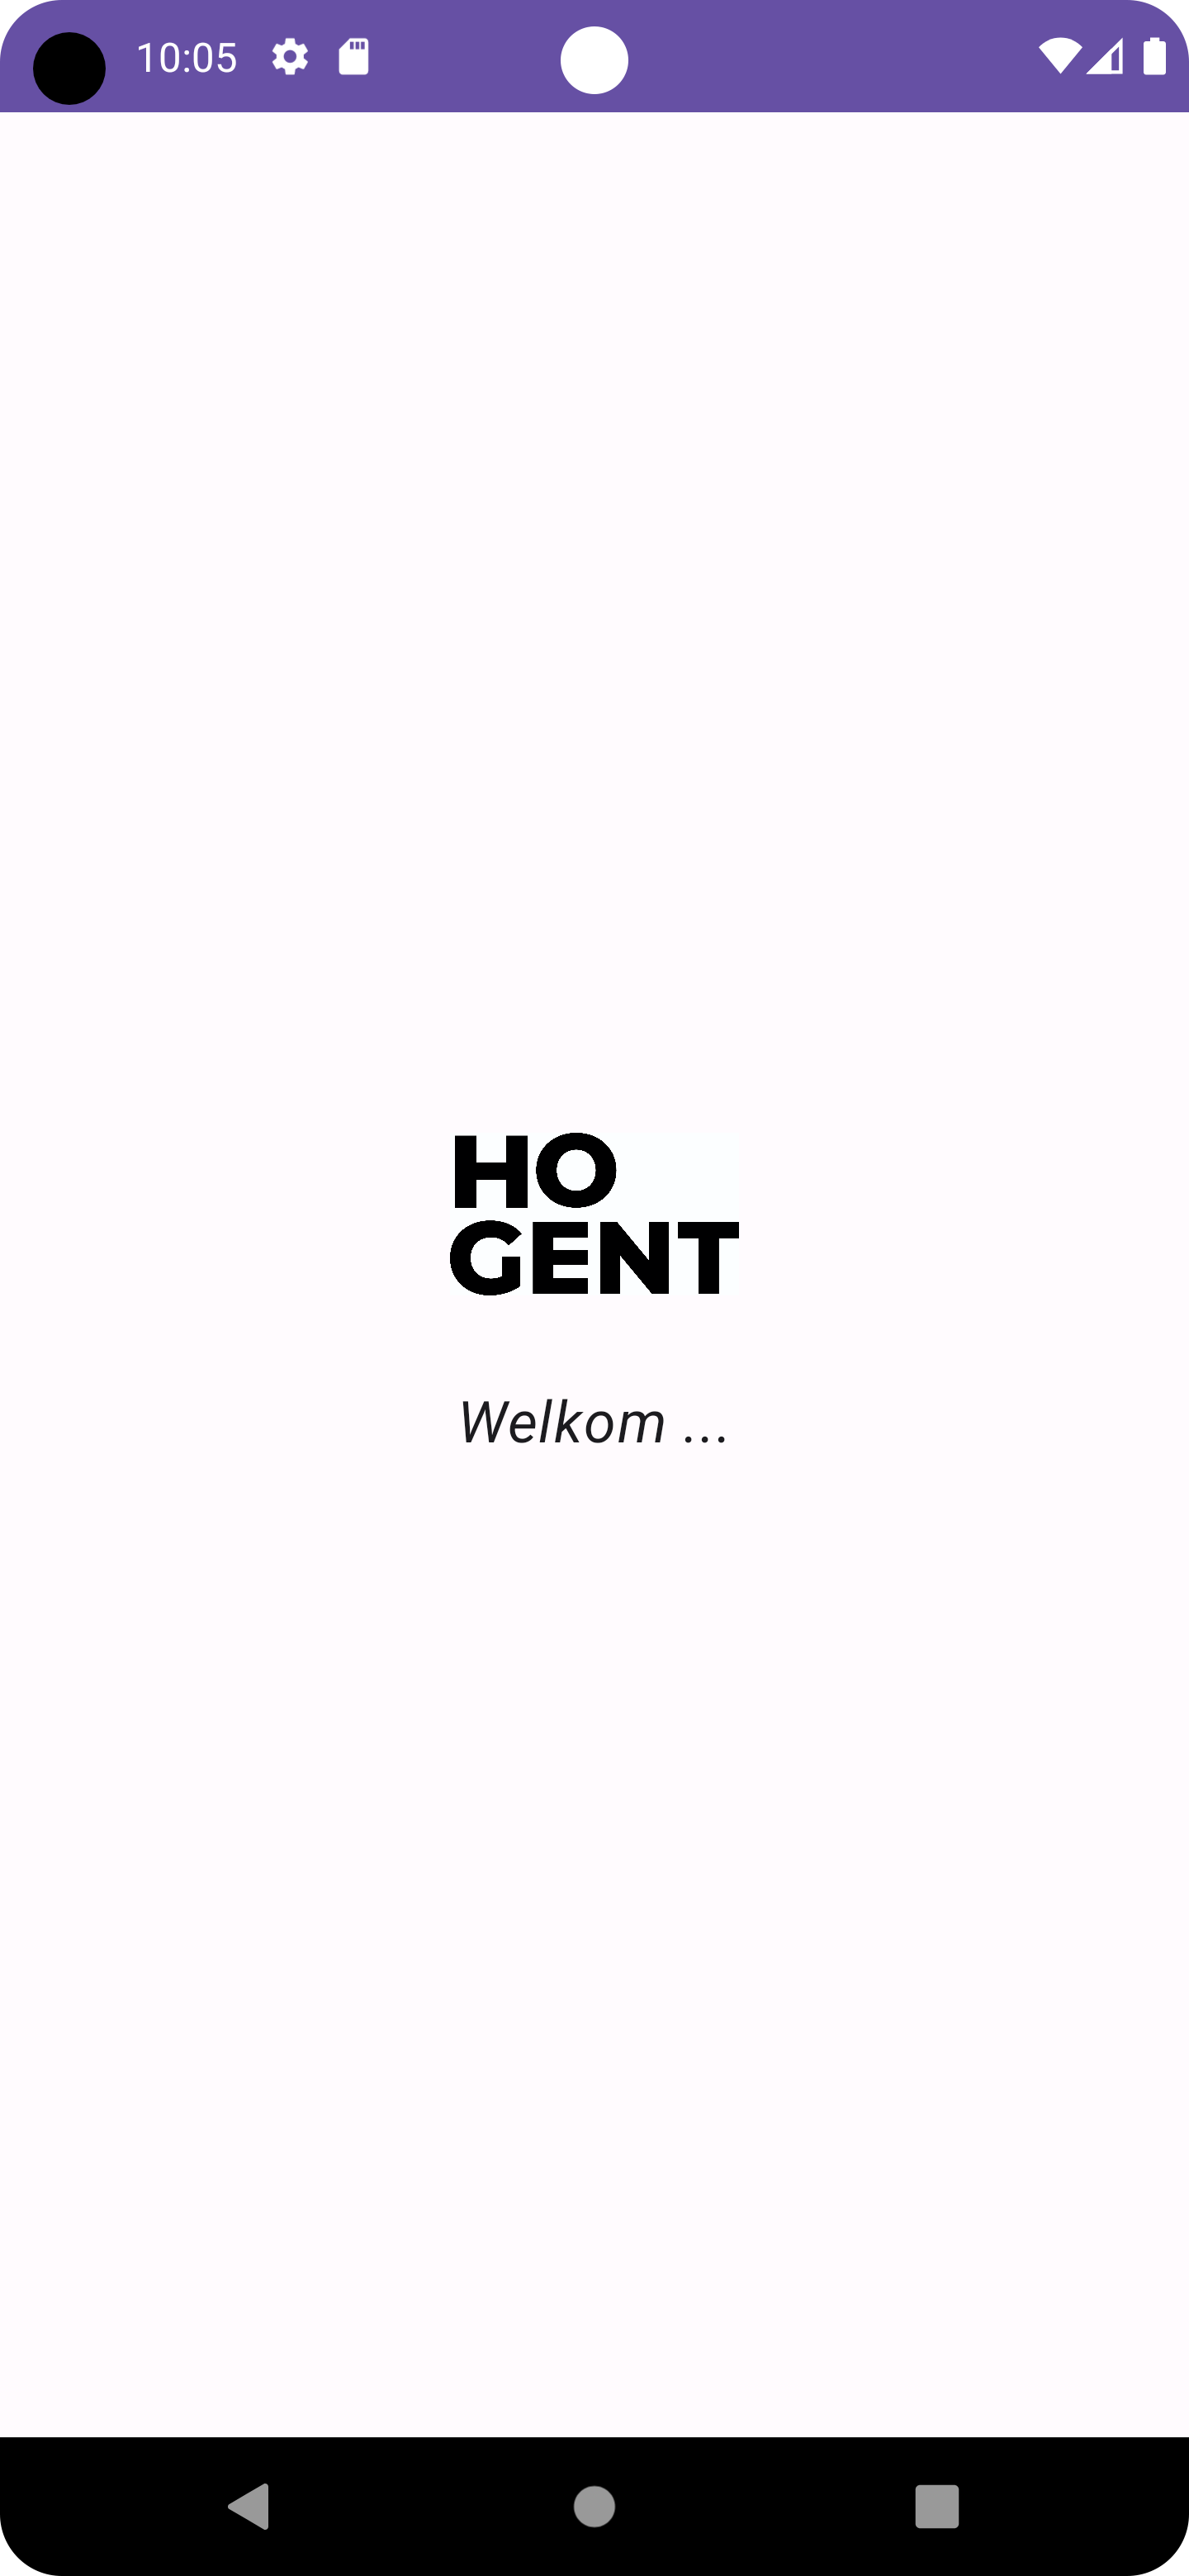
\includegraphics[width=0.5\textwidth]{mobile_intro.png}
    \captionsetup{justification=centering}
    \caption{Opstart van de mobiele applicatie: Toont het initiële laadscherm van de applicatie}
    \label{fig:mobile_intro}
\end{figure}

\begin{figure}[h]
    \centering
    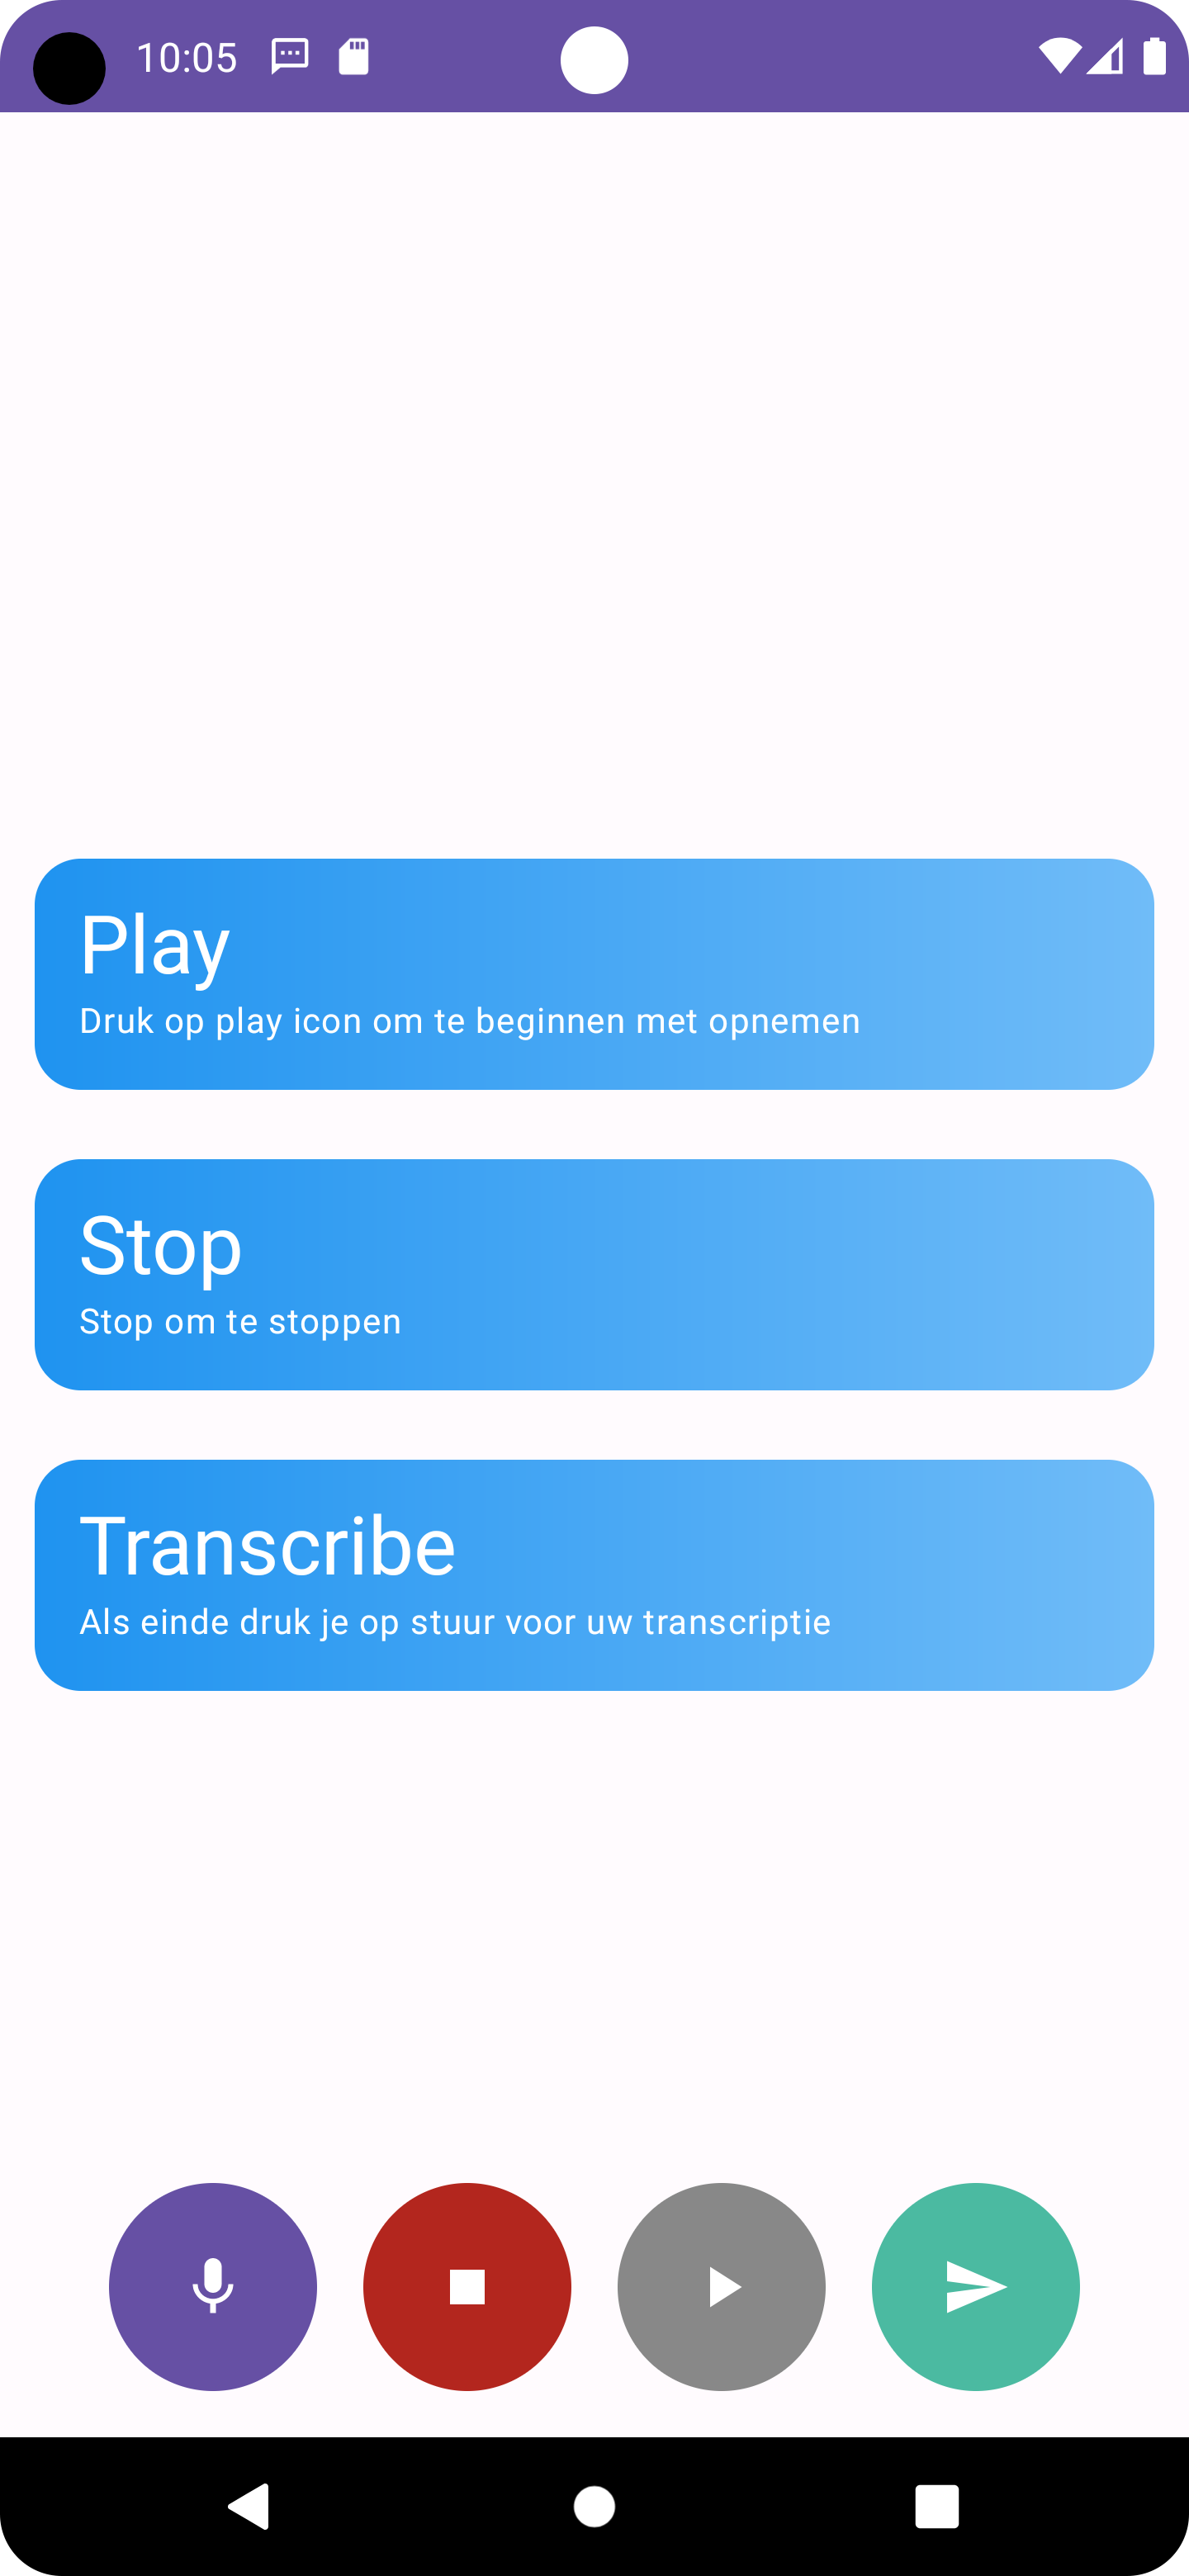
\includegraphics[width=0.5\textwidth]{mobile_home.png}
    \captionsetup{justification=centering}
    \caption{Hoofdscherm van de mobiele applicatie: Toont het centrale menu en biedt uitleg over het gebruik van de app.}    \label{fig:mobile_intro}
\end{figure}

\begin{figure}[h]
    \centering
    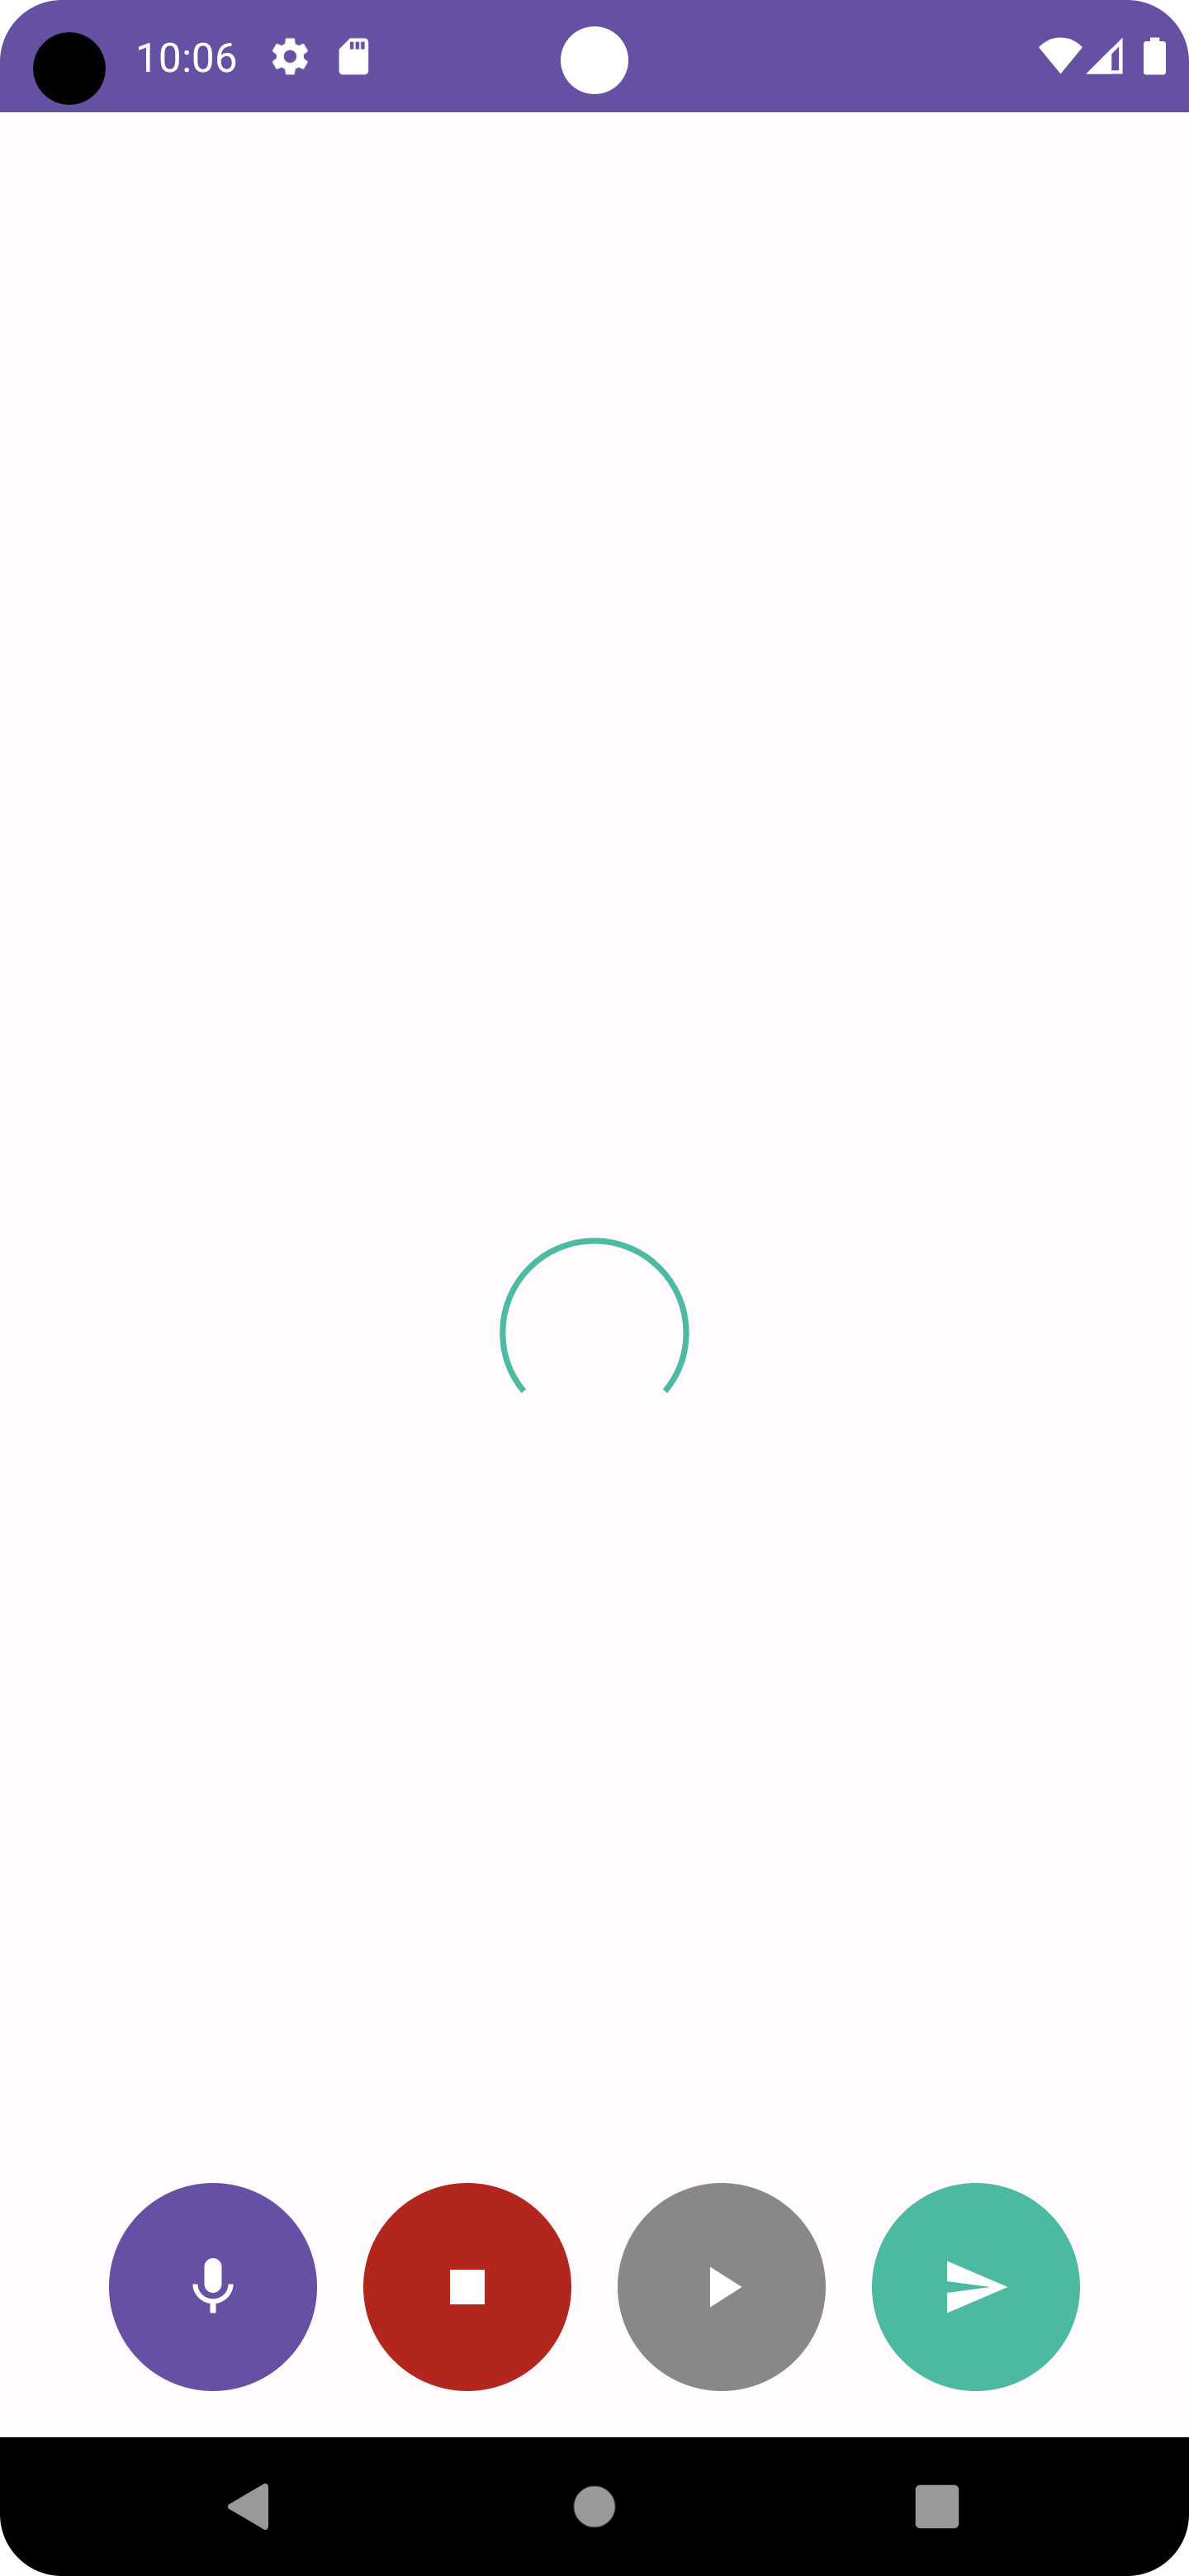
\includegraphics[width=0.5\textwidth]{mobile_loading.png}
    \captionsetup{justification=centering}
    \caption{Aanvraag laden: Illustreert de interface tijdens een gegevensaanvraag, verbetert de feedback voor gebruikers door een laadspinner te tonen.}
    \label{fig:mobile_intro}
\end{figure}

\begin{figure}[h]
    \centering
    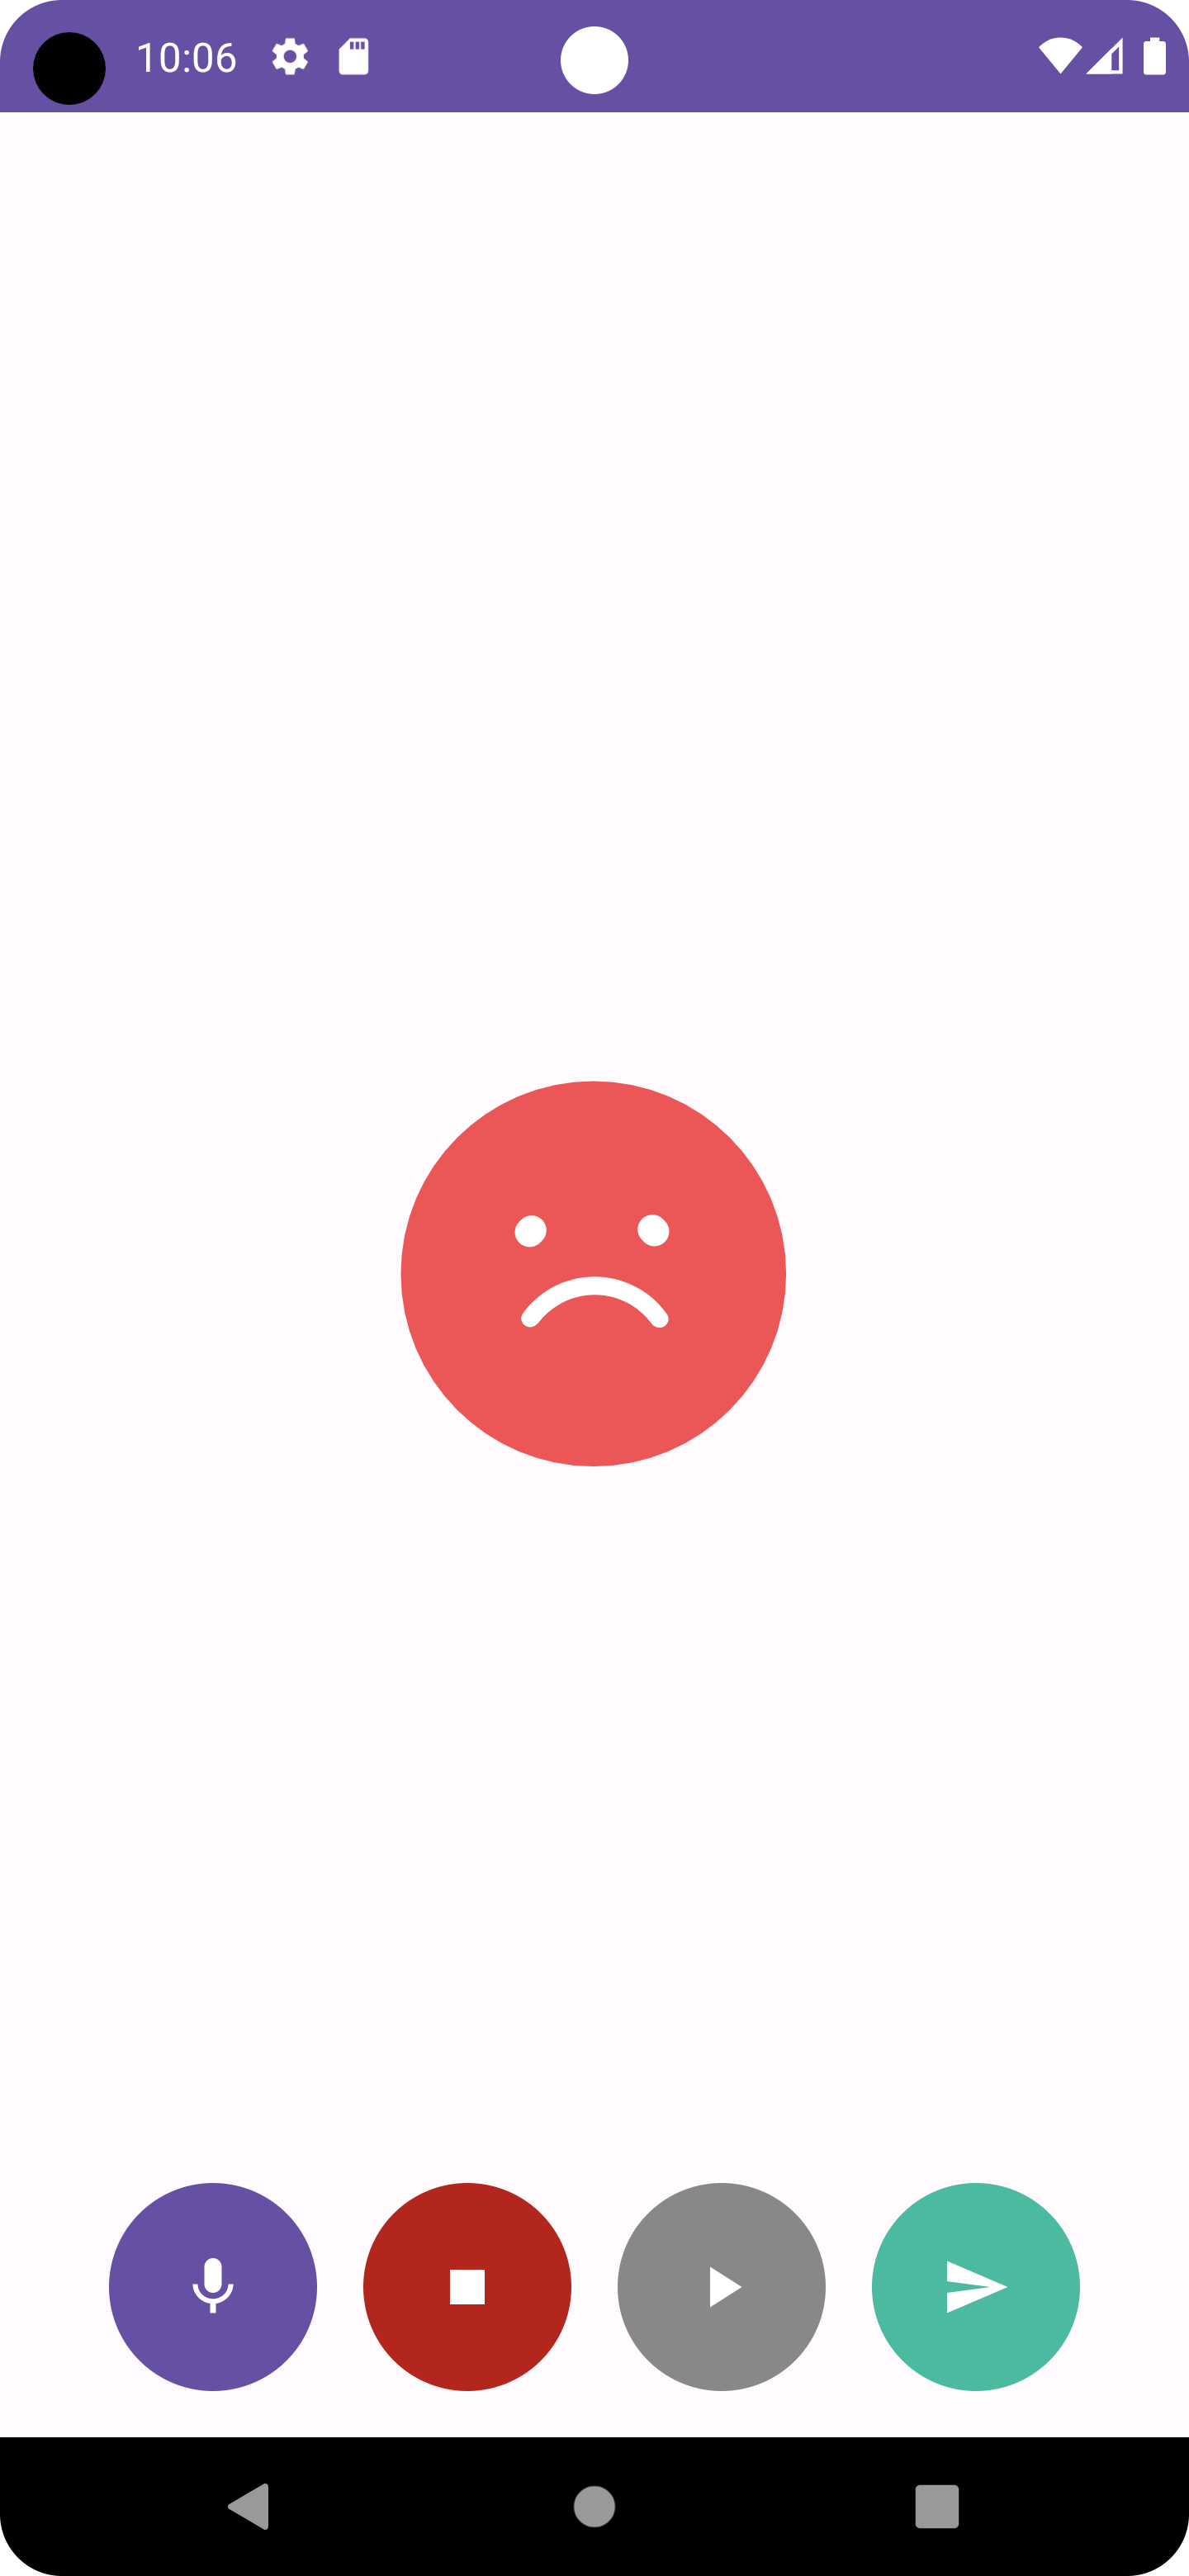
\includegraphics[width=0.5\textwidth]{mobile_badrequest.png}
    \captionsetup{justification=centering}
    \caption{Foutieve aanvraag: Legt de UI-reactie vast op een onsuccesvolle interactie met de server, en geeft gebruikers richtlijnen over mogelijke stappen om het probleem op te lossen.}
    \label{fig:mobile_intro}
\end{figure}
\FloatBarrier 
\section{Back-end Structuur}
Het project, SecondaryBabyTalkMonitorApi, is ontwikkeld om de communicatie tussen zorgverleners en oudere patiënten te analyseren door middel van spraakherkenning en linguïstische analyse. De structuur van de API is systematisch georganiseerd binnen een Java Spring Boot framework, wat efficiënte request handling en service management faciliteert.

De kernfunctionaliteit is ondergebracht in verschillende packages die elk een specifiek aspect van de applicatie adresseren. De `controller` package bevat de `TranscriptionController` die verantwoordelijk is voor het verwerken van audiofile uploads en het initiëren van de transcriptieprocessen. De `service` package omvat de `TranscriptionService` die gebruik maakt van een AI-client, gegenereerd door de `AiClientFactory`, om audio naar tekst te transcriberen via de AssemblyAI-API.

De `model` package bevat de `TranscriptionResponse` klasse die de resultaten van de transcripties opslaat, waaronder successtatus, volledige transcriptie, en sets van specifieke woorden zoals verkleinwoorden en nietzeggende woorden.


De `utility` package bevat de `LinguisticAnalysis` klasse, die essentieel is voor de linguïstische analyse van transcripties. Deze klasse is specifiek ontworpen om patronen zoals verkleinwoorden en herhalende zinnen te detecteren, welke indicatief zijn voor 'secondary babytalk'. De algoritmen die gebruikt worden voor deze identificatie zijn gebaseerd op eerder onderzoek  \autocite{Sibian2024} dat de kenmerkende elementen van 'secondary babytalk' heeft vastgesteld. Door deze geavanceerde analytische benaderingen te integreren, kan de klasse effectief bijdragen aan het ontrafelen van complexe taalpatronen die vaak voorkomen in de communicatie met oudere patiënten.

Deze API is bijzonder nuttig voor het identificeren van 'secondary babytalk' kenmerken in de communicatie, een essentiële factor voor het verbeteren van de interactie tussen zorgverleners en oudere patiënten. Dit alles toont een goed doordachte structuur die gericht is op het verbeteren van de zorgkwaliteit door geavanceerde technologieën in de linguïstiek en machine learning te integreren.
De volledige broncode van de backend is beschikbaar in de GitHub repository \textcite{AitCheikhAhmedBackEnd}.
\section{Hosting backend}
\begin{figure}[h]
    \centering
    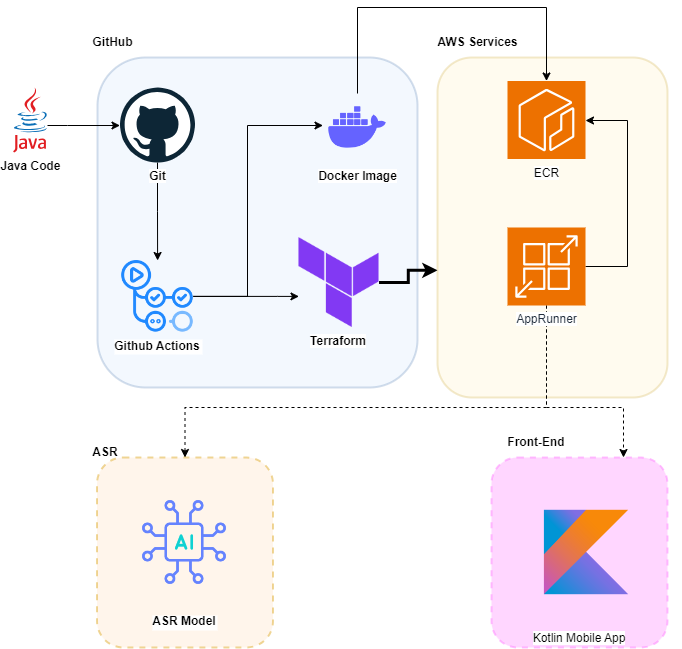
\includegraphics[width=0.8\textwidth]{architectuur_diagram.png}
    \captionsetup{justification=centering}
    \caption{Architectuur diagram van het project}
    \label{fig:architectuur}
\end{figure}
\FloatBarrier 
Het architectuurdiagram \ref{fig:architectuur} beschrijft hoe de baby-monitor POC is opgeboud, waarbij gebruik wordt gemaakt van zowel cloudgebaseerde diensten als geautomatiseerde workflows. Het hart van dit systeem is GitHub, gebruikt voor versie-controle met Git en voor het opslaan van Java-code, wat de basis vormt voor de applicatieontwikkeling.
\\
De integratie en levering van updates worden geautomatiseerd door GitHub Actions, terwijl Terraform zorgt voor de provisioning van AWS-resources. Dit omvat het creëren van Docker-images die worden beheerd in Amazon Elastic Container Registry (ECR) en uitgerold via AWS AppRunner, wat het beheer en de schaalbaarheid van de applicatie vereenvoudigt.

Daarnaast bevat het diagram een specifieke verwijzing naar een automatisch spraakherkenningsmodel (ASR) en een front-end ontwikkeld in Kotlin voor mobiele apparaten. Deze combinatie biedt een robuuste en gebruikersvriendelijke mobiele ervaring, geoptimaliseerd door de naadloze integratie van spraakgestuurde functies en efficiënte cloudservices.











